\section{Ziel}
Ziel dieses Versuchs ist es, die Magnetfelder von verschiedenen
Spulen und ihre Eigenschaften zu untersuchen und zu bestimmen. %zu ähnlich wie die Anleitung?

\section{Theorie}
\label{sec:Theorie}

%\cite{V308}

\subsection{Allgemeine Grundlagen zu spulenerzeugten Magnetfeldern } %"Magnetfelder von Spulen"?
Die magnetische Flussdichte $\symbf{B}$ wird durch die Permeabilität $\mu$ und die 
magnetische Feldstärke $\symbf{H}$ dargestellt. Es gilt die Beziehung 
\begin{equation} 
    \symbf{B} = \mu \cdot \symbf{H}.
    \label{eqn:B}
\end{equation}
$\mu$ besteht dabei aus der Vakuum-Permeabilität $\mu_{0}$ und der relativen 
Permeabilität $\mu_{r}$, die von der Materie abhängt. 
Es gilt 
\begin{equation*} 
    \mu = \mu_{0} \cdot \mu_{r}.
\end{equation*}
\newline
%KURZE SPULE:
Die magnetische Flussdichte im Mittelpunkt einer Spule wird mit der Formel 
\begin{equation}
    \symbf{B}(x)= n \cdot \frac{\mu_{0} I}{2} \frac{R^2}{(R^2 +x^2)^{3/2}}\cdot \symbf{\hat{x}}
    \label{eqn:kurzespule}
\end{equation}
beschrieben. 
Dabei ist $R$ der Radius des Rings, $n$ die Anzahl der Windungen, $I$ die Stromstärke von der die Spule durchflossen wird und $x$ die Position auf der Achse.
Der Vektor $\symbf{\hat{x}}$ ist die normierte Richtungsableitung, wobei hier nur der Betrag des Vektors $\symbf{B}$ betrachtet wird.
\newline
%LANGE SPULE:
Bei einer langen Spule (Solenoid) ist die magnetische Flussdichte in der Mitte der 
Spule konstant. Außerhalb der Spule ist der magnetische Fluss inhomogen. 
Das innere Feld ist antiproportional zur Länge $l$ der Spule und proportional zur Anzahl der Windungen %antiproportional zu l oder nicht? 
$n$ und zum Strom $I$, der durch die Spule fließt. 
Es gilt die Beziehung
\begin{equation}
    B = \mu_{r} \mu_{0} \frac{n}{l} I.
    \label{eqn:langespule}
\end{equation}
%SPULENRING:
Wird dieser Solenoid zu einem Ring mit Radius $r_{R}$ gebogen, verschwinden die 
Randeffekte und das Feld außerhalb des Rings wird null. 
Im Inneren gilt
\begin{equation}
    B = \mu_{r} \mu_{0} \frac{n}{2\pi r_{R}} I.
    \label{eqn:ring}
\end{equation}
Wegen Gleichung \eqref{eqn:B} muss für das $H$-Feld gelten:
\begin{equation}
    H = \frac{n}{2\pi r_{R}} I.
    \label{eqn:H}
\end{equation}

\subsection{Magnetfeld eines Spulenpaares}
Ein Helmholtz-Spulenpaar hat ein annähernd homogenes Magnetfeld im Innern der zwei Spulen %Spulen statt Ringe
(s. Abb \ref{fig:helmholtz}). Der Abstand der Spulen entspricht bei einem Helmholtz-Spulenpaar den Radien der
Spulen.
Die magnetische Flussdichte im Mittelpunkt eines allgemeinen Spulenpaares ist durch 
\begin{equation}
    B(0)= B_{n}(x) + B_{n}(-x) = n \frac{\mu_{0} I R^2}{(R^2 + x^2)^{3/2}} %mal 2n oder n??????????? ich glaub nur n. ist ja in beiden Spulen gleich und wenn man dann beide Spulen addiert zieht man das n einfach raus aus der Summe. Deshalb nur ein n. Passt auch besser zu unseren Theoriewerten. 
    \label{eqn:spulenpaar}
\end{equation}
gegeben.
\begin{figure}
    \centering
    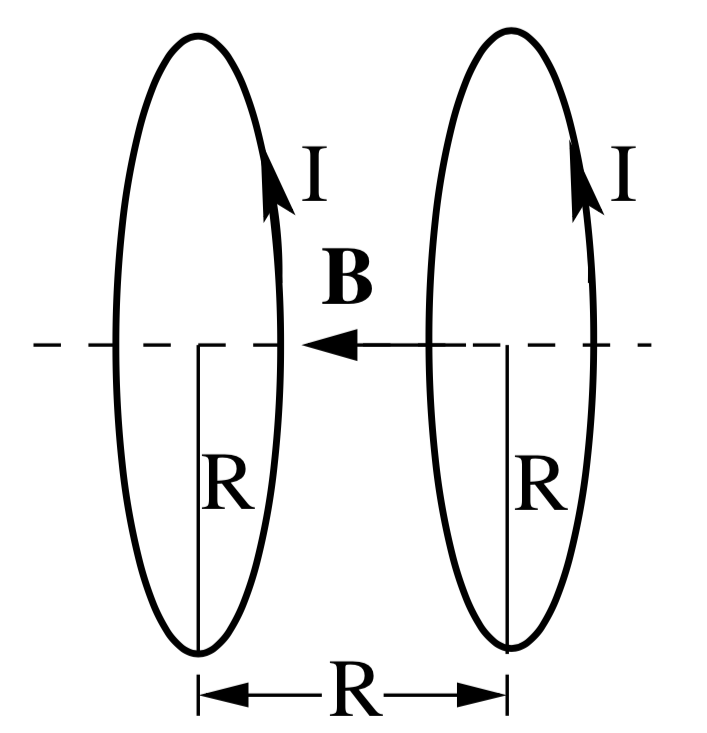
\includegraphics[width=8cm,height=6cm]{build/Helmholtz.png}%nicht hübsch, nochmal gucken mit den Werten
    \caption{Aufbau eines Helmholtz-Spulenpaares. Der Abstand der Spulen
    entspricht den Radien der Spulen.}
    \label{fig:helmholtz}
\end{figure}

\subsection{Ferromagnetismus und die Hysteresekurve}
Ferromagnetische Materialien besitzen ohne äußere Magnetfelder ein permanentes 
magnetisches Moment. Sie richten sich in einzelnen Bereichen parallel zueinander aus. 
Man nennt diese Bereiche Weiß'sche Bezirke. Im unmagnetischen Zustand ist die 
Ausrichtung der Bereiche statistisch verteilt. Ein äußeres Magnetfeld sorgt für eine 
Änderung der Richtung der magnetischen Momente und vergrößert somit die Weiß'schen 
Bereiche. 
\newline
Die relative Permeabilität $\mu_{r}$ ist in ferromagnetischen Materialien sehr hoch 
und ist nicht mehr linear proportional zur magnetischen Flussdichte. 
Die Abhängigkeit kann durch eine Hysteresekurve dargestellt werden.
Dabei sind die Achsen das $B$- und das $H$-Feld.
In der Kurve lassen sich verschiedene markante Punkte erkennen. 
Ohne äußeres Magnetfeld gilt $B = H = 0$. Wird ein Magnetfeld angelegt, steigt die 
Magnetisierung an, bis ein Sättigungswert $B_{S}$ bei $H_{S}$ erreicht wird. Der 
Kurvenverlauf dorthin wird Neukurve (1) genannt. 
Wird das äußere Magnetfeld verringert, bilden sich Bereiche mit entgegengesetzer 
Magnetisierung. So bleibt, wenn das äußere Magnetfeld abgeschaltet wird, eine 
Restmagnetisierung $B_{r}$, genannt Remanenz, bestehen. 
Ein Gegendfeld $H$ kann diese Ausrichtungen wieder 
aufheben (2), sodass die magnetische Flussdichte beim Erreichen der sogenannten Koerzitivkraft $H_C$ Null wird. Wenn dieses Feld noch weiter 
erhöht wird, wird die magnetische Flussdichte %Magnetisierung oder magnetische Flussdichte? Magnetisierung ist doch schon negativ gewesen.
in dem Stoff negativ und erreicht den Sättigungswert $-B_{S}$. Wird das äußere 
Magnetfeld wieder umgekehrt (3), entsteht eine zum Ursprung punktsymmetrische Kurve, welche
Hysteresekurve genannt wird. Hysteresekurven verschiedener Stoffe unterscheiden sich je
nach Materialeigenschaften in der Schärfe bzw. Breite. 
\begin{figure}
    \centering
    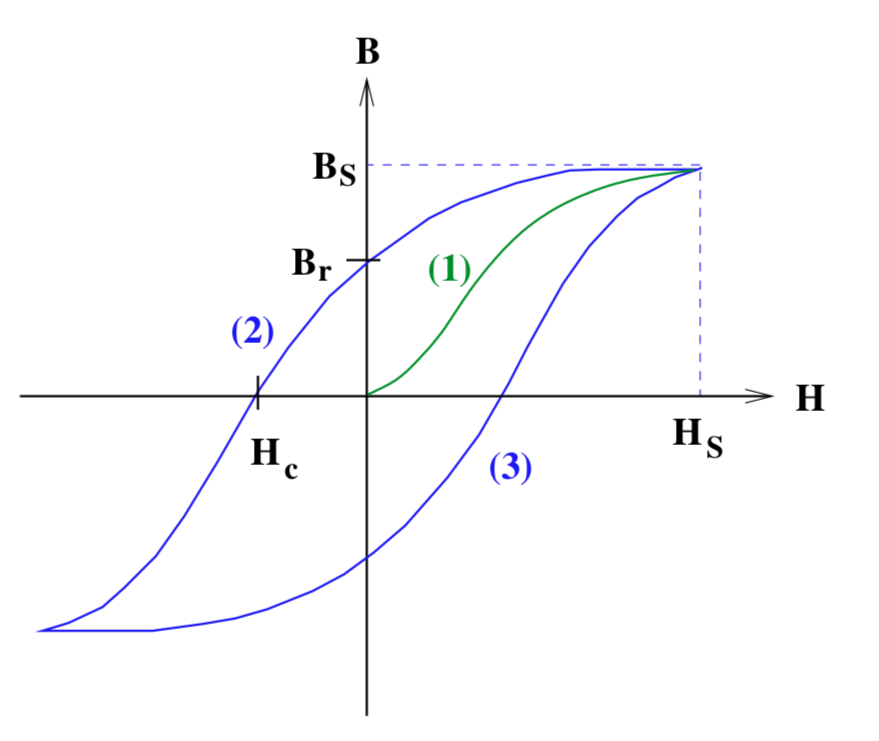
\includegraphics[width=10cm,height=10cm]{build/Hysteresekurve.png}
    \caption{Allgemeine Hysteresekurve. Eingezeichnet sind der Sättigungswert $B_{S}$
    sowie $H_{S}$, die Remanenz $B_{r}$ und die Koerzitivkraft $H_{c}$.}
\end{figure}
